\documentclass[11pt]{article}

% ---------------------------------------------------------------------------
% Handout: Recursive reversal -> additive displacement
% Compile:  module load texlive/2025 && pdflatex displacement_handout.tex
%           (run twice; forest/tikz need a second pass)
% ---------------------------------------------------------------------------

\usepackage[margin=2.1cm]{geometry}
\usepackage{amsmath,amssymb}
\usepackage{xcolor}
\usepackage{tikz}
\usetikzlibrary{positioning,calc,arrows.meta,decorations.pathreplacing,fit,backgrounds}
\usepackage{forest}
\usepackage[most]{tcolorbox}
\usepackage{booktabs}
\usepackage{parskip}
\usepackage{microtype}

% --- palette ---------------------------------------------------------------
\definecolor{headc}{HTML}{1B7F3B}   % head child  (green)
\definecolor{compc}{HTML}{1F5FBF}   % complement child (blue)
\definecolor{flipc}{HTML}{C0392B}   % flip node (red)
\definecolor{invc}{HTML}{555555}    % invariant / stationary (gray)
\definecolor{panel}{HTML}{F4F1EA}

\newcommand{\head}[1]{\textcolor{headc}{#1}}
\newcommand{\comp}[1]{\textcolor{compc}{#1}}
\newcommand{\flip}[1]{\textcolor{flipc}{#1}}
\newcommand{\swap}{\ensuremath{\mathbin{\textcolor{flipc}{\rightleftarrows}}}}

% --- callout boxes ---------------------------------------------------------
\newtcolorbox{rulebox}[1][]{colback=panel,colframe=black!70,boxrule=0.6pt,
  arc=2pt,left=6pt,right=6pt,top=4pt,bottom=4pt,title=#1,fonttitle=\bfseries}
\newtcolorbox{keybox}[1][]{colback=flipc!6,colframe=flipc!75,boxrule=0.8pt,
  arc=2pt,left=6pt,right=6pt,top=4pt,bottom=4pt,title=#1,fonttitle=\bfseries}

% --- forest style: highlight flip nodes ------------------------------------
\forestset{
  default preamble={
    for tree={font=\small, edge={-, gray}, l sep=10pt, s sep=7pt,
              inner sep=1.6pt, align=center}
  },
  flip/.style={draw=flipc, very thick, rounded corners=2pt, text=flipc},
  inv/.style ={draw=invc!55, thick, rounded corners=2pt, text=invc},
  leaf/.style={font=\small\itshape, text=black},
}

% --- token-flow diagram helper --------------------------------------------
% \tokflow{dx}{ HI list }{ HF list }{ arc list }
%   HI/HF list entries:  index/label   HF label may repeat words freely.
%   arc list entries:    hiIndex/hfSlot/colorname/labeltext
\newcommand{\tokflow}[4]{%
\begin{tikzpicture}[
   tok/.style={draw=black!55, fill=white, rounded corners=1.5pt,
               minimum height=6.5mm, inner xsep=3pt, font=\footnotesize},
   every node/.style={anchor=center}]
  \def\dx{#1}
  % top row = HI
  \foreach \i/\lab in {#2}{ \node[tok] (hi\i) at (\i*\dx,2.35) {\lab}; }
  % bottom row = HF
  \foreach \m/\lab in {#3}{ \node[tok] (hf\m) at (\m*\dx,0) {\lab}; }
  \node[font=\scriptsize\bfseries, text=invc] at (-1.05,2.35) {HI};
  \node[font=\scriptsize\bfseries, text=invc] at (-1.05,0)    {HF};
  % arcs
  \foreach \a/\b/\c/\t in {#4}{
     \draw[\c, line width=1.1pt, -{Stealth[length=4pt]}, opacity=0.9]
        (hi\a.south) to[out=-90,in=90] node[midway, sloped, above=-1pt,
        font=\tiny, text=\c]{\t} (hf\b.north);
  }
\end{tikzpicture}}
% -------------------------------------------------------------------------

\newcommand{\rightm}{headc}   % right-mover color alias
\newcommand{\leftm}{compc}

\begin{document}

\begin{center}
  {\LARGE\bfseries From Recursive Reversal to Additive Displacement}\\[2pt]
  {\large How ``head-initial $\to$ head-final'' becomes a permutation you compute by \emph{counting}}\\[2pt]
  {\small Handout for the RASP-L construction \; (\texttt{experiments/22\_rasp\_l\_hi\_hf})}
\end{center}

\vspace{-3pt}
\hrule
\vspace{6pt}

\noindent
Head-final (HF) reorders a head-initial (HI) sentence by reversing the two children of
certain \emph{flip} nodes, recursively. That sounds like it needs a full tree walk. This
handout shows the shortcut: each token's final position is its start position \emph{plus a
sum of independent shifts}, one per flip node it sits inside. Every example below is
machine-verified against the grammar's own generator.

% ==========================================================================
\section*{1.\quad Setup: HF is a permutation, driven by \emph{flip} nodes}

Every HI/HF rule keeps the \emph{same words}, only reordered, so HF is a permutation of HI.
A node either \flip{\textbf{flips}} its two children (\head{head} $\;\leftrightarrow\;$
\comp{complement} swap order) or is \textcolor{invc}{\textbf{invariant}} (children keep
order). The \swap{} marks flip nodes.

\begin{center}
\begin{minipage}{0.46\textwidth}\centering
\begin{forest}
[S, inv
  [DP, inv[{John},leaf]]
  [{VP\,\swap}, flip
    [V[{likes},leaf]]
    [DP, inv [D[{the},leaf]] [NP[{dog},leaf]]]
  ]
]
\end{forest}\\[2pt]
{\footnotesize HI: \emph{John likes the dog}}
\end{minipage}\hfill
\begin{minipage}{0.5\textwidth}
{\footnotesize
\textbf{\flip{Flip}} (reverse HI$\to$HF):\\
\quad \texttt{CP\_sent}=[\head{C}\,$|$\,\comp{S}], \;
      \texttt{CP\_rel}=[\head{C}\,$|$\,\comp{S\_gap}],\\
\quad \texttt{VP}=[\head{V(+Adv)}\,$|$\,\comp{obj/clause}],\\
\quad \texttt{NP\_singular}=[\head{noun}\,$|$\,\comp{rel.\ clause}].\\[3pt]
\textbf{\textcolor{invc}{Invariant}} (keep order):\\
\quad \texttt{S}=[subj$|$VP], \; \texttt{DP}=[D$|$N],\\
\quad \texttt{NP\_singular\_adj}=[Adj$|$N], \; \texttt{S\_obj\_gap}=[DP$|$V].
}
\end{minipage}
\end{center}

% ==========================================================================
\section*{2.\quad One flip $=$ a block swap}

A flip node lays its children out as two adjacent blocks and swaps them:

\begin{center}
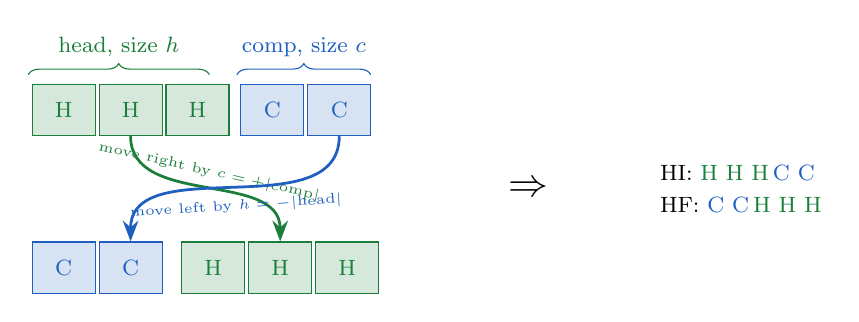
\begin{tikzpicture}[box/.style={draw, minimum width=8mm, minimum height=6.5mm},
                    every node/.style={font=\footnotesize}]
  % top (HI): H H H  C C
  \foreach \i in {0,1,2}{\node[box, fill=headc!18, draw=headc] (h\i) at (\i*0.85,1.6){\head{H}};}
  \foreach \i in {0,1}  {\node[box, fill=compc!18, draw=compc] (c\i) at (2.65+\i*0.85,1.6){\comp{C}};}
  \draw[decorate,decoration={brace,amplitude=4pt},headc] (-0.45,2.05)--(1.85,2.05)
       node[midway,above=3pt]{\head{head, size $h$}};
  \draw[decorate,decoration={brace,amplitude=4pt},compc] (2.2,2.05)--(3.9,2.05)
       node[midway,above=3pt]{\comp{comp, size $c$}};
  % bottom (HF): C C  H H H
  \foreach \i in {0,1}  {\node[box, fill=compc!18, draw=compc] (bc\i) at (\i*0.85,-0.4){\comp{C}};}
  \foreach \i in {0,1,2}{\node[box, fill=headc!18, draw=headc] (bh\i) at (1.9+\i*0.85,-0.4){\head{H}};}
  % arrows
  \draw[headc,-{Stealth},line width=1pt] (h1.south) to[out=-90,in=90]
       node[midway,sloped,font=\tiny,above]{move right by $c=+|\text{comp}|$} (bh1.north);
  \draw[compc,-{Stealth},line width=1pt] (c1.south) to[out=-90,in=90]
       node[midway,sloped,font=\tiny,below]{move left by $h=-|\text{head}|$} (bc1.north);
  \node at (5.9,0.6){\Large$\Rightarrow$};
  \node[align=left,font=\footnotesize] at (8.6,0.6)
    {HI: \head{H H H}\,\comp{C C}\\[2pt] HF: \comp{C C}\,\head{H H H}};
\end{tikzpicture}
\end{center}

\begin{keybox}[The whole rule (one flip)]
\vspace{-3pt}
\[
 \text{disp}(x)=
 \begin{cases}
   +\,|\text{comp}| & \text{if } x \text{ is in the \head{head} child (jumps right over the complement)}\\[2pt]
   -\,|\text{head}| & \text{if } x \text{ is in the \comp{complement} child (jumps left over the head)}
 \end{cases}
\]
\vspace{-8pt}
\end{keybox}

\noindent\textbf{Worked, \emph{John likes the dog}} \;($\text{VP}=[\head{likes}\mid\comp{the\ dog}]$,
so $|\text{head}|=1,\ |\text{comp}|=2$):

\begin{center}
\tokflow{1.9}
  {0/John, 1/likes, 2/the, 3/dog}
  {0/John, 1/the, 2/dog, 3/likes}
  {0/0/invc/0, 1/3/headc/{+2}, 2/1/compc/{-1}, 3/2/compc/{-1}}
\end{center}

\begin{rulebox}[A second way to read the numbers -- ``who crosses over me''?]
$\text{disp}(x)=\big(\#\text{ tokens on }x\text{'s \emph{right} in HI that land \emph{left} of it in HF}\big)-\big(\#\text{ that go the other way}\big)$.
For a \head{head} token, its \emph{entire} complement sits to its right and all of it crosses left $\Rightarrow +|\text{comp}|$.
For a \comp{complement} token, the \emph{entire} head sits to its left and crosses right $\Rightarrow -|\text{head}|$.
This ``count the crossers'' view is exactly what the transformer computes with an attention head.
\end{rulebox}

% ==========================================================================
\section*{3.\quad Nesting is \emph{additive} (the key idea)}

When flips nest, a token's displacement is just the \textbf{sum} of one contribution per
enclosing flip -- no interaction terms. Why:

\begin{keybox}[Why it adds]
An \textbf{inner} flip only rearranges tokens \emph{within its own span}. An \textbf{outer}
flip then picks up that entire span and slides it \emph{rigidly} -- every token inside moves
by the \emph{same} amount. So each nesting level contributes an independent offset, and they
stack:\quad
$\text{disp}(x)=\displaystyle\sum_{\substack{F\text{ a flip node}\\ \text{enclosing } x}}
\big(\,{+}|\text{comp}(F)|\ \text{if }x\in\head{\text{head}(F)},\ \ {-}|\text{head}(F)|\ \text{if }x\in\comp{\text{comp}(F)}\,\big).$
\end{keybox}

\begin{center}
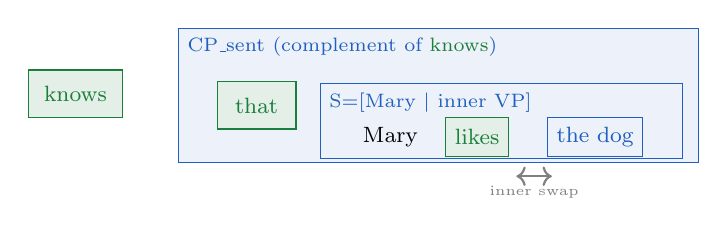
\begin{tikzpicture}[font=\footnotesize]
  \node[draw=headc, fill=headc!12, minimum width=1.2cm, minimum height=6mm] (kn) at (0,0){\head{knows}};
  \node[draw=compc, fill=compc!8, minimum width=6.6cm, minimum height=1.7cm, anchor=west] (cp) at (1.3,-0.02){};
  \node[anchor=north west, compc, font=\scriptsize] at (cp.north west){\comp{CP\_sent} (complement of \head{knows})};
  \node[draw=headc, fill=headc!12, minimum width=1cm, minimum height=6mm] (th) at (2.3,-0.15){\head{that}};
  \node[draw=compc, fill=compc!8, minimum width=4.6cm, minimum height=0.95cm, anchor=west] (s) at (3.1,-0.35){};
  \node[anchor=north west, compc, font=\scriptsize] at (s.north west){\comp{S}=[Mary $|$ inner VP]};
  \node[minimum height=5mm] (mary) at (4.0,-0.55){Mary};
  \node[draw=headc, fill=headc!12, minimum height=5mm] (li) at (5.1,-0.55){\head{likes}};
  \node[draw=compc, fill=compc!8, minimum height=5mm] (td) at (6.6,-0.55){\comp{the dog}};
  \draw[<->, gray, thick] (5.6,-1.05) -- (6.05,-1.05) node[midway,below,font=\tiny]{inner swap};
\end{tikzpicture}
\end{center}

\noindent\textbf{Worked, \emph{John knows that Mary likes the dog}} -- three nested flips
$\text{VP}\supset\text{CP\_sent}\supset\text{VP}$:

\begin{center}
\begin{minipage}{0.44\textwidth}\centering
\begin{forest}
[S, inv
 [DP,inv[{John},leaf]]
 [{VP\,\swap},flip
  [V[{knows},leaf]]
  [{CP\_sent\,\swap},flip
   [C[{that},leaf]]
   [S,inv
    [DP,inv[{Mary},leaf]]
    [{VP\,\swap},flip
      [V[{likes},leaf]]
      [DP,inv[D[{the},leaf]][N[{dog},leaf]]]
    ]
   ]
  ]
 ]
]
\end{forest}
\end{minipage}\hfill
\begin{minipage}{0.54\textwidth}
\small
\begin{tabular}{@{}rll r@{}}
\toprule
tok & contributions & $=$disp & hf\\
\midrule
John  & (none)                                   & $0$  & 0\\
\head{knows} & \head{$+5$}\,(VP.head)                    & $+5$ & 6\\
that  & $-1$(VP.c) \; \head{$+4$}(CP.head)       & $+3$ & 5\\
Mary  & $-1$(VP.c) \; $-1$(CP.c)                  & $-2$ & 1\\
likes & $-1$(VP.c) \; $-1$(CP.c) \; \head{$+2$}(VP.head) & $0$ & 4\\
the   & $-1$ \; $-1$ \; $-1$                     & $-3$ & 2\\
dog   & $-1$ \; $-1$ \; $-1$                     & $-3$ & 3\\
\bottomrule
\end{tabular}
\end{minipage}
\end{center}

\begin{center}
\tokflow{1.75}
  {0/John, 1/knows, 2/that, 3/Mary, 4/likes, 5/the, 6/dog}
  {0/John, 1/Mary, 2/the, 3/dog, 4/likes, 5/that, 6/knows}
  {0/0/invc/0, 1/6/headc/{+5}, 2/5/headc/{+3}, 3/1/compc/{-2}, 4/4/invc/0, 5/2/compc/{-3}, 6/3/compc/{-3}}
\end{center}

\noindent Read the \emph{likes} row: it is the head of the \emph{inner} VP ($+2$), but that whole
inner clause is also the complement of \texttt{CP\_sent} ($-1$) and of the matrix \texttt{VP}
($-1$). The three shifts sum to $0$. The embedded subject \emph{Mary} sits under the invariant
\texttt{S}, so it is never a flip-head/comp itself -- it only collects the two $-1$ pushes from
the flips it is \emph{nested in}. \textbf{Subjects only ever get pushed left, never swapped.}

% ==========================================================================
\section*{4.\quad The recipe: computing an offset by hand}

Everything above collapses into a four-step crank you can run on any sentence, without ever
simulating the recursive reversal:

\begin{rulebox}[Compute $\text{disp}(x)$ in four steps]
\begin{enumerate}\setlength{\itemsep}{2pt}
\item \textbf{Tag the tree.} Mark each internal node a \flip{flip} (\texttt{VP} with an overt
  complement, \texttt{CP\_sent}, \texttt{CP\_rel}, or \texttt{NP\_singular} carrying a relative
  clause) or \textcolor{invc}{\textbf{invariant}} (\texttt{S}, \texttt{DP},
  \texttt{S\_subj\_gap}, \texttt{S\_obj\_gap}).
\item \textbf{Size each flip.} Record $|\head{\text{head}}|$ and $|\comp{\text{comp}}|$, in tokens.
\item \textbf{Collect contributions.} For a token $x$, walk \emph{every} flip $F$ whose span
  \emph{contains} $x$ (not only its parent) and add
  \[
    \head{+\,|\text{comp}(F)|}\ \text{ if } x\in\head{\text{head}(F)},
    \qquad
    \comp{-\,|\text{head}(F)|}\ \text{ if } x\in\comp{\text{comp}(F)}.
  \]
\item \textbf{Sum and shift.} $\text{disp}(x)=\sum_F(\cdots)$, then
  $\text{hf\_pos}(x)=\text{hi\_pos}(x)+\text{disp}(x)$; the output is the gather
  $\text{out}[j]=\text{hi}[\,x:\text{hf\_pos}(x)=j\,]$.
\end{enumerate}
\end{rulebox}

\noindent The single place this goes wrong by hand is step~3's \emph{contains} vs.\ \emph{is a
child of}: a token pays into \emph{every} flip it sits inside, because an outer flip picks up the
inner span and slides it \emph{rigidly} (\S3) -- so an inner token inherits the outer $\pm$
unchanged. Two consequences worth memorizing: a \textbf{subject} sits under an invariant
\texttt{S}, so it is never any flip's head or complement -- it only ever \emph{collects} the
$-|\head{\text{head}}|$ pushes of the flips it is nested in (always leftward, never a swap); and a
token can be a flip's \head{head} yet still not move, when the outer $-$ pushes exactly cancel its
inner $+$ (the \emph{likes} row above: $\head{+2}\,{-}1\,{-}1=0$).

\begin{center}\footnotesize
\emph{Warm-up (one flip).} \quad ``\emph{Mary likes the dog}'', $\text{VP}=[\head{likes}\mid\comp{the\ dog}]$:
\end{center}
\vspace{-6pt}
\begin{center}
\tokflow{1.9}
  {0/Mary, 1/likes, 2/the, 3/dog}
  {0/Mary, 1/the, 2/dog, 3/likes}
  {0/0/invc/0, 1/3/headc/{+2}, 2/1/compc/{-1}, 3/2/compc/{-1}}
\end{center}

% ==========================================================================
\section*{5.\quad Same rule, a different flip: relative clauses}

\textbf{\emph{the boy that chases the dog swims}} -- the outermost flip is
$\text{NP\_singular}=[\head{boy}\mid\comp{that\ chases\ the\ dog}]$, so the relative clause
jumps in \emph{front} of the noun it modifies.

\begin{center}
\begin{minipage}{0.5\textwidth}\centering
\begin{forest}
[S,inv
 [DP,inv
  [D[{the},leaf]]
  [{NP\,\swap},flip
   [N[{boy},leaf]]
   [{CP\_rel\,\swap},flip
    [C[{that},leaf]]
    [S\_subj\_gap,inv
     [{VP\,\swap},flip
       [V[{chases},leaf]]
       [DP,inv[D[{the},leaf]][N[{dog},leaf]]]
     ]
    ]
   ]
  ]
 ]
 [VP,inv[V[{swims},leaf]]]
]
\end{forest}
\end{minipage}\hfill
\begin{minipage}{0.48\textwidth}
\small
\begin{tabular}{@{}rll r@{}}
\toprule
tok & contributions & $=$disp & hf\\
\midrule
the    & (none)                              & $0$  & 0\\
\head{boy} & \head{$+4$}(NP.head)                & $+4$ & 5\\
that   & $-1$(NP.c) \; \head{$+3$}(CPrel.head)& $+2$ & 4\\
chases & $-1$ \; $-1$ \; \head{$+2$}(VP.head) & $0$  & 3\\
the    & $-1$ \; $-1$ \; $-1$                 & $-3$ & 1\\
dog    & $-1$ \; $-1$ \; $-1$                 & $-3$ & 2\\
swims  & (none)                              & $0$  & 6\\
\bottomrule
\end{tabular}
\end{minipage}
\end{center}

\begin{center}
\tokflow{1.75}
  {0/the, 1/boy, 2/that, 3/chases, 4/the, 5/dog, 6/swims}
  {0/the, 1/the, 2/dog, 3/chases, 4/that, 5/boy, 6/swims}
  {0/0/invc/0, 1/5/headc/{+4}, 2/4/headc/{+2}, 3/3/invc/0, 4/1/compc/{-3}, 5/2/compc/{-3}, 6/6/invc/0}
\end{center}

\noindent\emph{the}(0) and \emph{swims}(6) don't move: the determiner sits in an invariant DP,
and the intransitive matrix verb has no complement to swap with. Same three-line rule, new node
labels.

% ==========================================================================
\section*{6.\quad Why this shape is perfect for a transformer}

\begin{rulebox}[From displacement to the program]
\vspace{-2pt}
\[
 \text{hf\_pos}(x) \;=\; \underbrace{\text{hi\_pos}(x)}_{\texttt{indices}}
 \;+\; \underbrace{\text{disp}(x)}_{\text{sum of }\pm|\text{sibling}|}
 \qquad\Longrightarrow\qquad
 \text{out}[j]=\text{hi}\big[\,x:\text{hf\_pos}(x)=j\,\big].
\]
\vspace{-9pt}
\end{rulebox}

\noindent The displacement gives each token an \emph{exact integer} target slot (a true
permutation -- no sorting), and the output is one inverse-permutation \emph{gather}. The only
thing the rule needs is, per token, the \textbf{sizes of the sibling constituents} of every
flip it sits inside -- i.e.\ the constituent \emph{spans}. Recovering spans from the flat string
is the bracket-matching in \textbf{Stage 2} of the program. Everything else -- reading a token's
head/complement role, and the final gather -- is elementwise maps, relative-position reads, and
counting: the length-generalizing core of RASP-L.

\vfill
\begin{center}\footnotesize\itshape
All examples verified against \texttt{grammar\_oracle.py}, which computes this displacement and
matches the v2 generator's \texttt{hf} column 100\% on depth-$\le 2$.
\end{center}

\end{document}
